\documentclass[12pt,a4paper]{article}
\usepackage{fontspec, xunicode, xltxtra}
\setmainfont{SimSun}
\usepackage{indentfirst} 
\setlength{\parindent}{2em}
\XeTeXlinebreaklocale "zh"
\usepackage[left=2.5cm,right=2.5cm,top=2.5cm,bottom=2.5cm]{geometry}
\usepackage{changepage}
\usepackage{float}
\usepackage{setspace}
\usepackage{amsmath}
\usepackage{amsfonts}
\usepackage{amssymb}
\usepackage{circuitikz}
\usepackage{graphicx}

\title{实验四\quad 波形发生电路}
\author{自54 田毅\\ 2015011451}

\graphicspath{{Figure/}}
\begin{document}
\begin{spacing}{1.3}
\maketitle
\tableofcontents
\newpage
\section{实验目的}
\begin{enumerate}
\item 掌握由集成运放构成的正弦波振荡电路的原理与参数选择方法。
\item 学习电压比较器的组成及电压传输特性的测试方法。
\item 掌握由集成运放构成的矩形波和三角波振荡电路的原理与参数选择方法。
\end{enumerate}
\section{预习报告}
\subsection{正弦波发生电路}
\subsubsection{理论估算}
\begin{figure}[H]
\centering
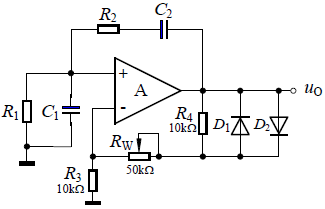
\includegraphics{1.jpg}
\end{figure}
如图,按文氏桥电路通常选择方式,选取$R_1=R_2=R,C_1=C_2=C$,则RC串并联选频网络确定的频率为: 
\[f_0=\frac{1}{2\pi RC},此时|\dot{F}|=\frac{1}{3}\]
运算放大器构成引入了电压串联负反馈的放大电路,在满足放大倍数大于3的条件下与选频网络构成了振荡电路的同时,还具有尽可能大的输入电阻和尽可能小的输出电阻,减小了放大电路对选频特性的影响。\par
为了使输出电压的频率$f_0=400Hz$,则$RC= 0.398ms。$结合元件取值,可以取$R=4k\Omega ,C=0.1\mu F$,
计算可得$f_0=397.9Hz$。
\subsubsection{仿真实验}
仿真电路如下图所示。
\begin{figure}[H]
\centering
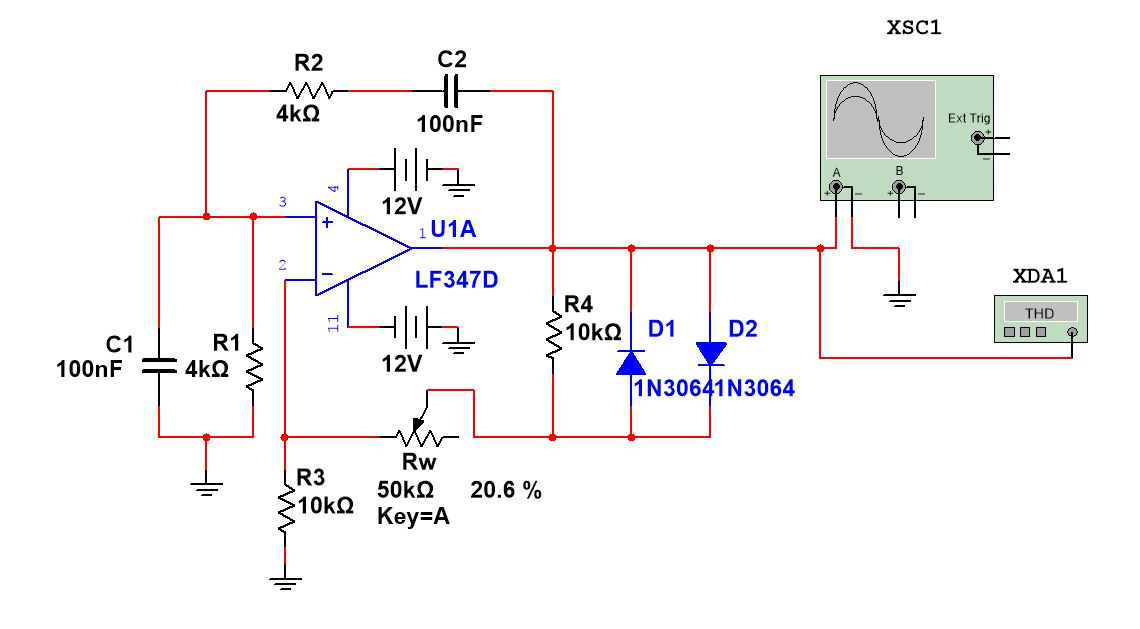
\includegraphics[width=\textwidth]{2.jpg}
\end{figure}
\paragraph{$R_w$为$0\Omega$时$U_o$的波形} 此时放大电路的放大倍数小于3,不满足放大条件,故不会起振,输出为0,波形如下:
\begin{figure}[H]
\centering
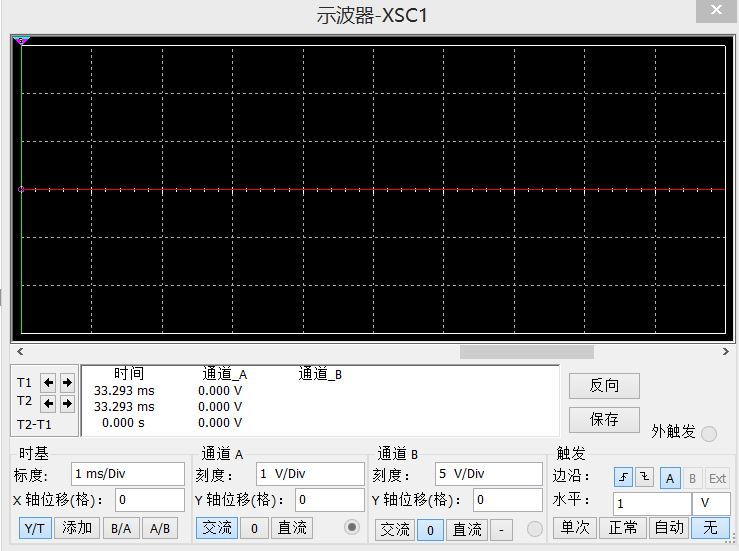
\includegraphics[width=\textwidth]{3.jpg}
\end{figure}
\paragraph{调整$R_w$使电路刚好起振,记录$U_o$的幅值、频率及$R_w$的阻值} 电路刚好起振时,$R_w = 50\times 20.8\% = 10.4k\Omega$,波形如下:
\begin{figure}[H]
\centering
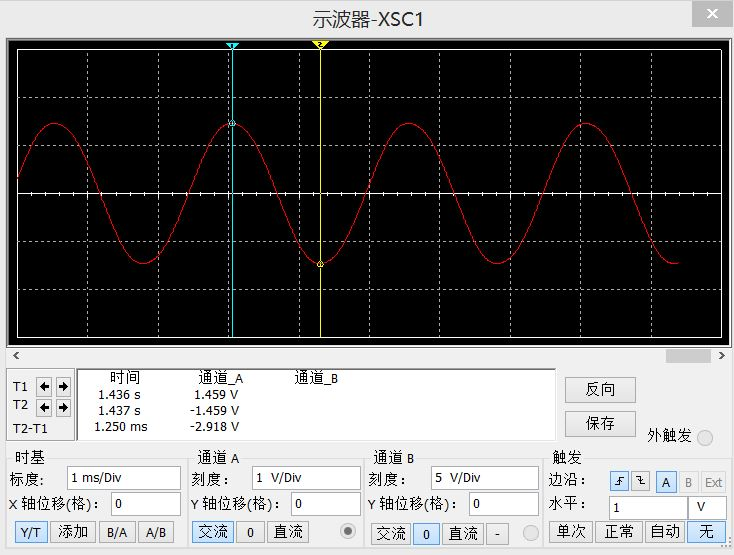
\includegraphics[width=\textwidth]{4-.jpg}
\end{figure}
测得输出电压的峰-峰值为$2.918V$,频率为$400Hz$。
此时没有明显失真现象。
\begin{figure}[H]
\centering
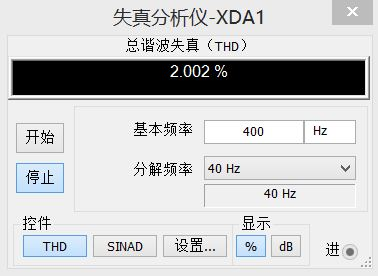
\includegraphics[width=8cm]{5-.jpg}
\end{figure}
\paragraph{调整$R_w$使输出为不失真的正弦波且幅值最大,记录$U_o$幅值、频率及$R_w$的阻值} 输出不失真且幅值最大时,$R_w = 50\times 36.0\% = 18.0k\Omega$,波形如下:
\begin{figure}[H]
\centering
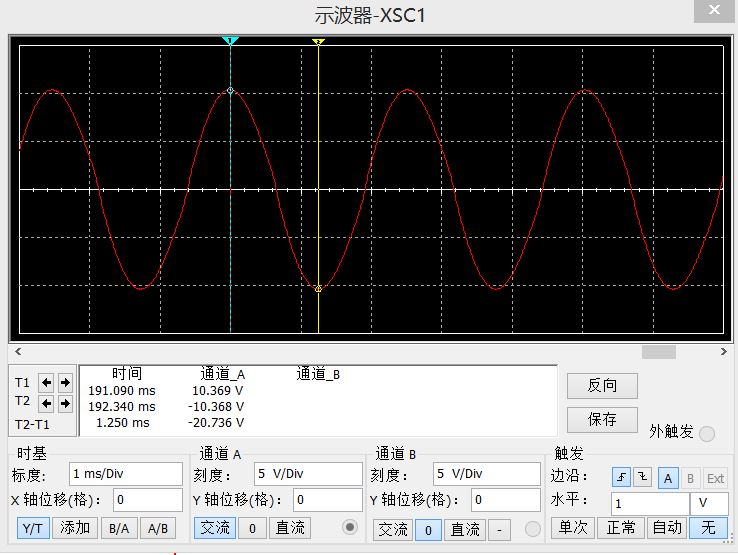
\includegraphics[width=\textwidth]{6-.jpg}
\end{figure}
可测得输出电压的峰-峰值为$20.736V$,频率为$400Hz$。此时没有明显的失真现象。
\begin{figure}[H]
\centering
\includegraphics[width=8cm]{6+.jpg}
\end{figure}
\paragraph{将两个二极管断开,观察$R_w$从小到大变化时输出波形的变化情况} $R_w$从小变大的过程中:
\begin{enumerate}
\item $R_w<=10.4k\Omega$时,没有产生振荡波形,或起振非常缓慢。
\item $R_w等于10.4k\Omega$时,电路开始振荡,且立刻达到顶部变平、失真的水平,如下图所示。
\begin{figure}[H]
\centering
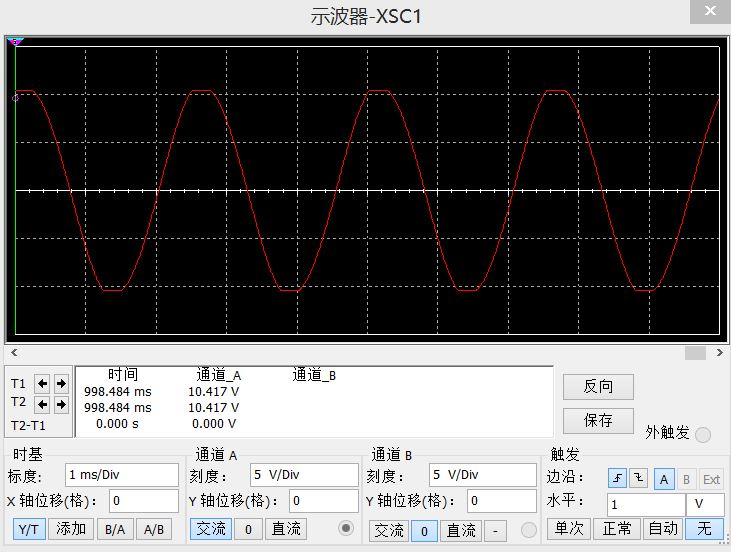
\includegraphics[width=\textwidth]{6-1.jpg}
\end{figure}
\item $R_w$稍微进一步增大时,输出波形出现失真,并且失真现象立刻非常严重,表现为与方波越来越接近。下图为$R_w=50\times 25\% = 12.5k\Omega$时的波形图。
\begin{figure}[H]
\centering
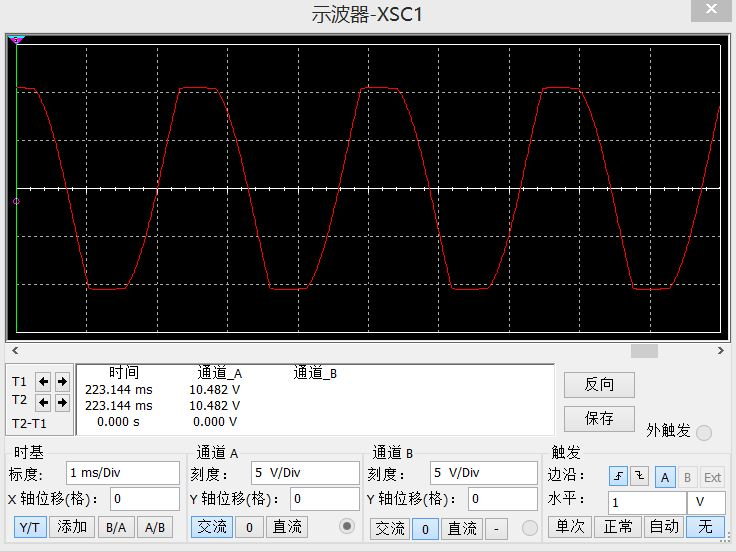
\includegraphics[width=\textwidth]{6-2.jpg}
\end{figure}
\end{enumerate}
\subsection{矩形波-三角波发生电路}
\subsubsection{理论估算}
\begin{figure}[H]
\centering
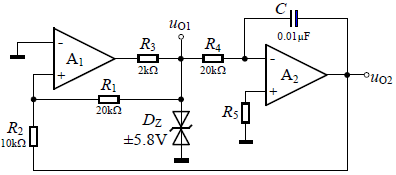
\includegraphics{7.jpg}
\end{figure}
\subsection{理论计算与分析}
在此电路中,左边为同相输入滞回比较器,阈值电压
\[\pm U_T = \pm \frac{R_2}{R_1}U_Z = \pm 2.9V\] \par
右边为积分运算电路。设初态时$u_{o1}为+U_Z$,则积分电路反向积分,$u_o$随时间的增长线性下降。当$u_{o2}=-U_T$时,再稍减小,$u_{o1}将从+U_Z跃变为-U_Z$,积分电路正向积分,$u_{o2}$随时间的增长线性上升。当$u_o=+U_T$时,再稍增加,$u_{o1}将从-U_Z跃变为+U_Z$,如此循环往复,产生自激振荡。故可见$u_{o1}$为幅值为$U_T$的方波,输出$u_{o2}$为为稳定的三角波,幅值为$U_Z$。\par 
由上述分析可知,正向积分的起始值为$-U_T$,终止值为$+U_T$,积分时间为二分之一周期,即
\[+U_T=\frac{1}{R_4 C} U_Z \cdot \frac{T}{2} -U_T \]
可解得振荡周期:
\[T=\frac{4R_2R_4C}{R_1}=0.4ms\]
\subsubsection{仿真实验}
仿真电路如下图所示。
\begin{figure}[H]
\centering
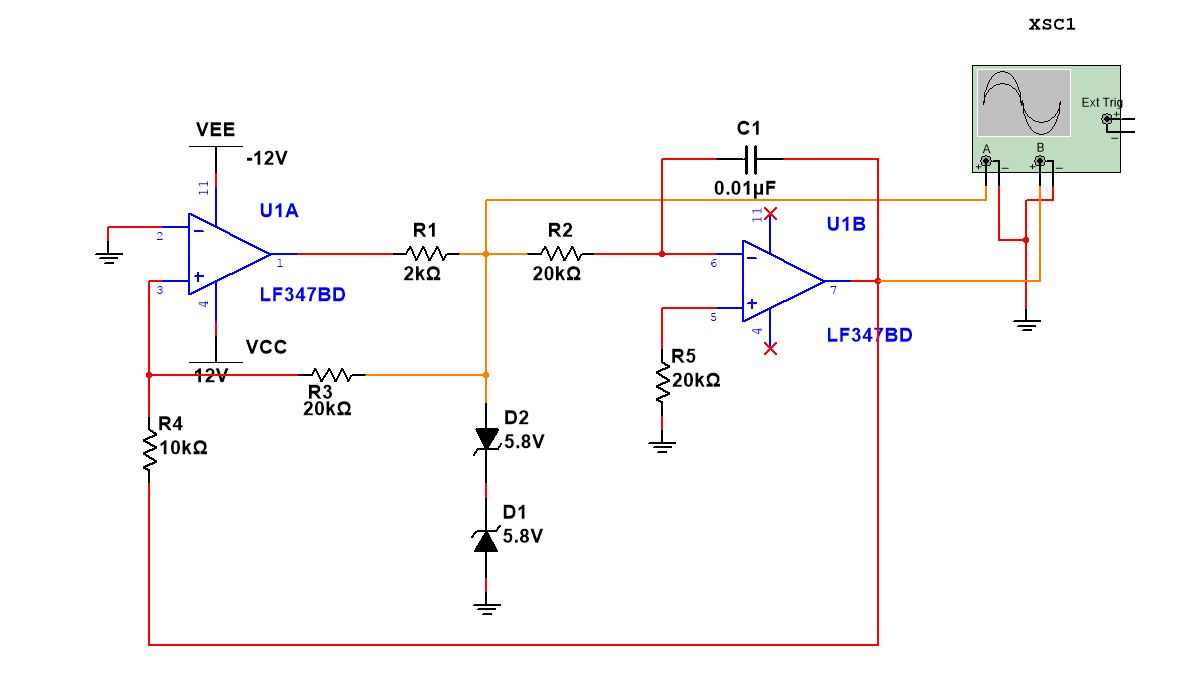
\includegraphics[width=\textwidth]{8-.jpg}
\end{figure}
仿真波形如下图所示。
\begin{figure}[H]
\centering
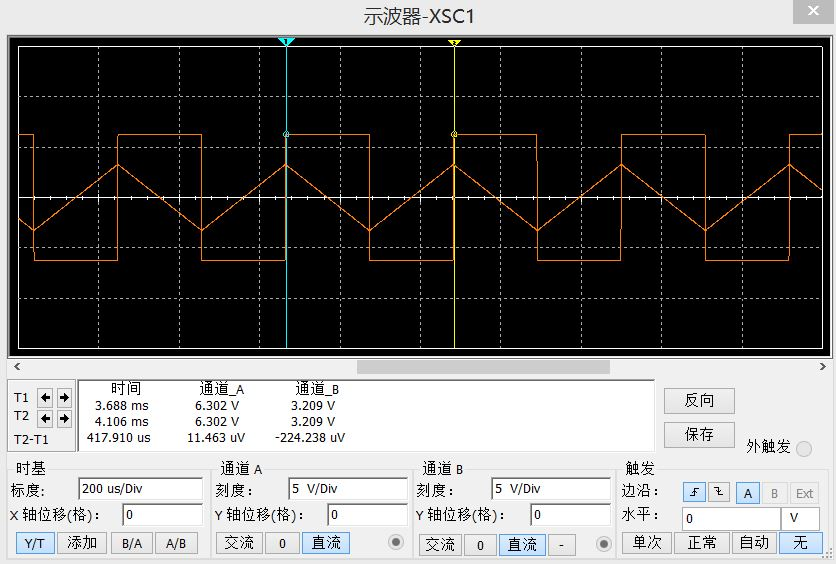
\includegraphics[width=\textwidth]{9-.jpg}
\end{figure}
可见$u_{o1}$的波形为方波,$u_{o2}$的波形为三角波,周期为$T=0.418ms$。\par
可用游标进一步测得$u_{o1}$的峰-峰值约为$12.581V$,$u_{o2}$的幅值约为$6.398V$,
$u_{o2}$的正程时间为$208.955ms$,逆程时间为$208.955m$。
\subsection{滞回比较器的电压传输特性}
测试时需将$R_2$与运放$A_2$的输出端断开,改接输入信号,输入信号可采用三角波。仿真电路如下图所示。
\begin{figure}[H]
\centering
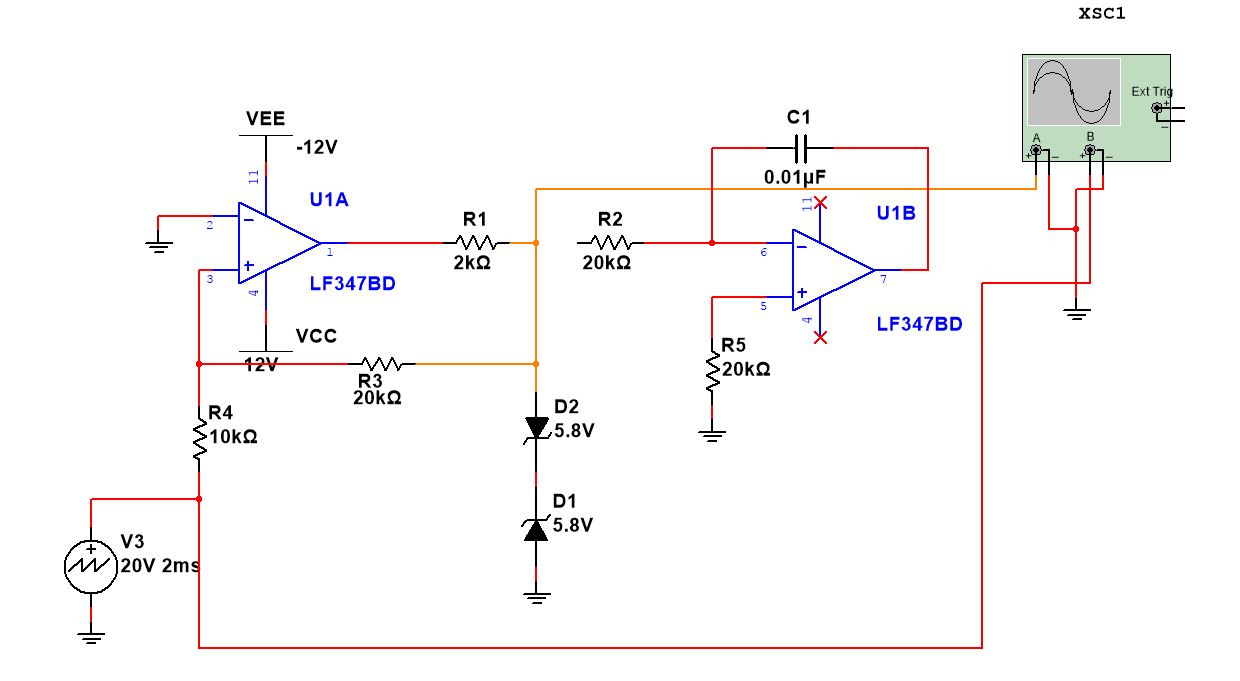
\includegraphics[width=\textwidth]{9-1.jpg}
\end{figure}
测量时将输入的三角波和$u_{o1}$接到示波器的两输入端并用$A/B$模式进行观察,可得到滞回比较电路的电压传输特性如下:
\begin{figure}[H]
\centering
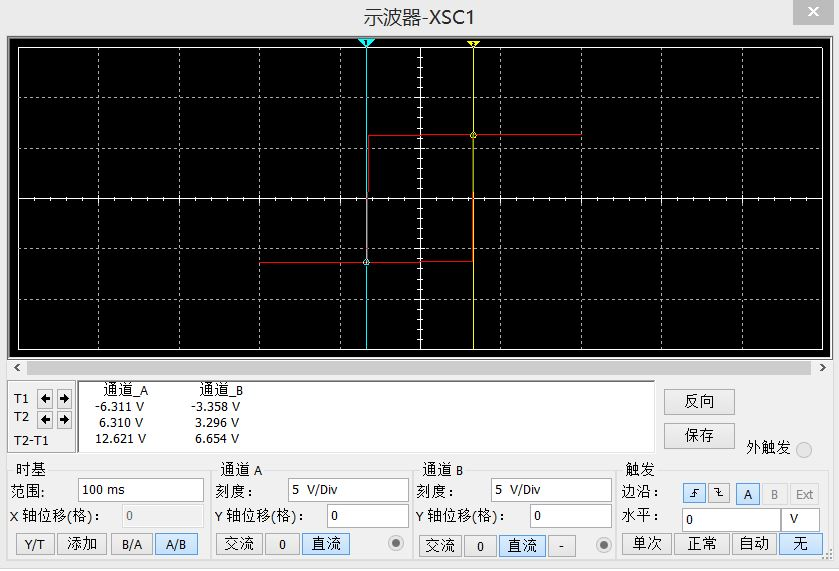
\includegraphics[width=\textwidth]{9-2.jpg}
\end{figure}
使用游标测得阈值电压平均值为$\frac{3.358+3.296}{2} = 3.327V$,$u_{o1}$的峰-峰值为$12.621V$。
\subsection{矩形波-锯齿波发生电路}
\subsubsection{理论估算}
只要使积分电路正向积分的时间常数和反向积分的时间常数的比值可以改变,就可得到占空比可调的锯齿波。基于这一想法,我们可以利用二极管的单向导电性,使积分电路两个方向的积分通路不同,从而实现题目的要求。
为了满足锯齿波的逆程时间大约是正程时间的$20\%$,需要正向积分的时间常数是反向的5倍,故若电容不变,反向通路中电阻应取$20\times 20\%=4k\Omega$。
\subsubsection{仿真实验}
\begin{figure}[H]
\centering
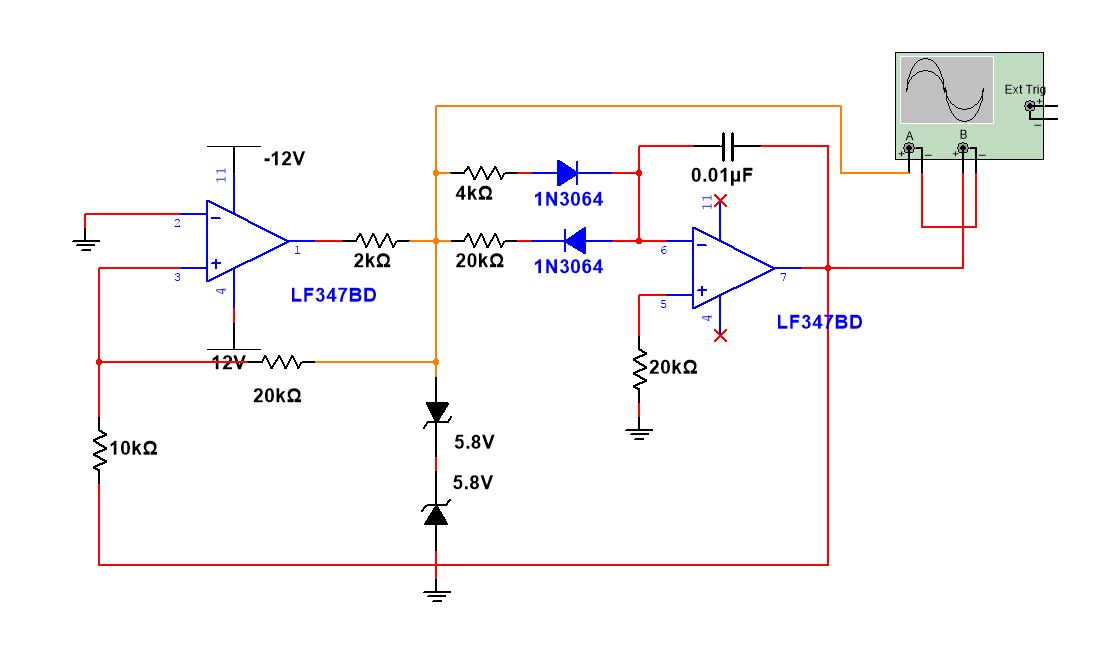
\includegraphics[width=\textwidth]{10-.jpg}
\end{figure}
波形如下,可见$u_{O1}$的波形为方波,$u_{O2}$的波形为锯齿波。
\begin{figure}[H]
\centering
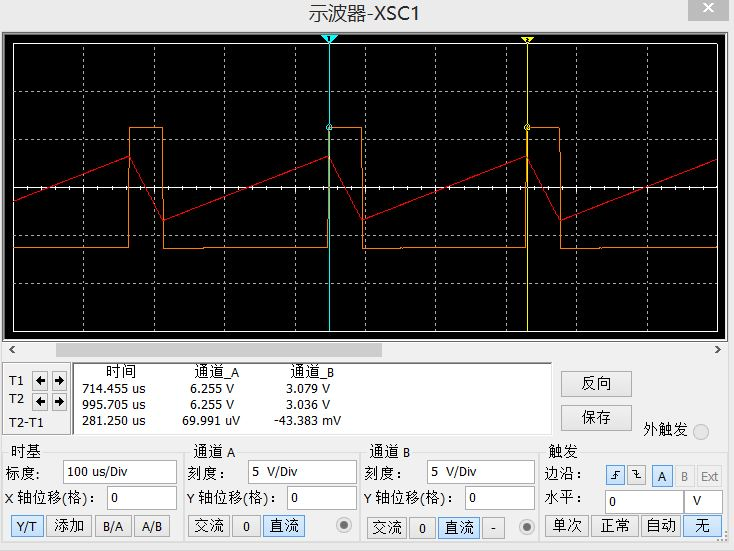
\includegraphics[width=\textwidth]{11-.jpg}
\end{figure}
可用游标测出
\[\frac{t_{逆程}}{t_{正程}} = \frac{48.295\mu s}{234.375\mu s} \approx 20.61\%\]
更进一步地,测得周期为$284.091\mu s$,$U_{o1}$的峰-峰值$12.126V$,$U_{o2}$的峰-峰值$6.508V$。
\section{注意事项}
\begin{enumerate}
\item 实验中要将学习机、信号源、示波器等电子仪器和实验电路共地,以免引起干扰。 
\item 请注意运算放大器LF347电源的正确接入,谨防因正负电源接反而烧坏芯片。
\end{enumerate}
\section{硬件实验}
\subsection{正弦波发生电路}
\subsubsection{$R_w$为$0\Omega$时$U_o$的波形}
\begin{figure}[H]
\centering
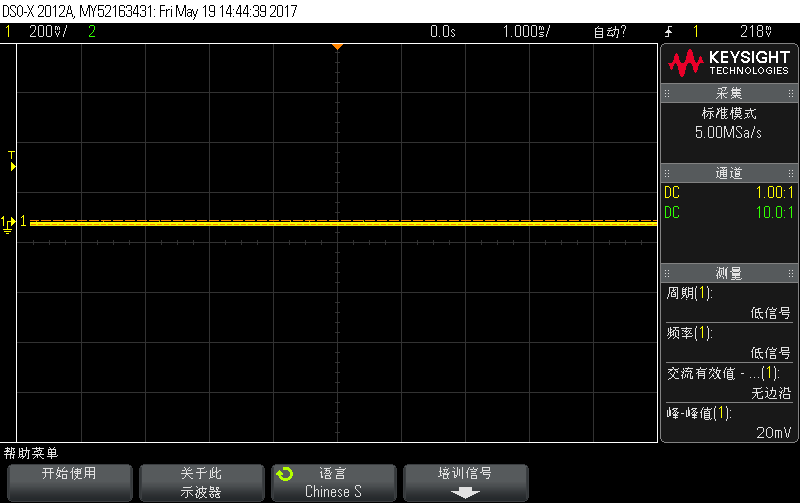
\includegraphics[width=\textwidth]{scope_0.png}
\end{figure}
\subsubsection{调整$R_w$使电路刚好起振,记录$U_o$的幅值、频率及$R_w$的阻值}
实验中$R_w为47k\Omega$的电位器,而实际选用的$R_1 = 39k\Omega , C = 10nF$。电路刚好起振时,用万用表电阻档测得$R_w = 9.91k\Omega$,波形如下:
\begin{figure}[H]
\centering
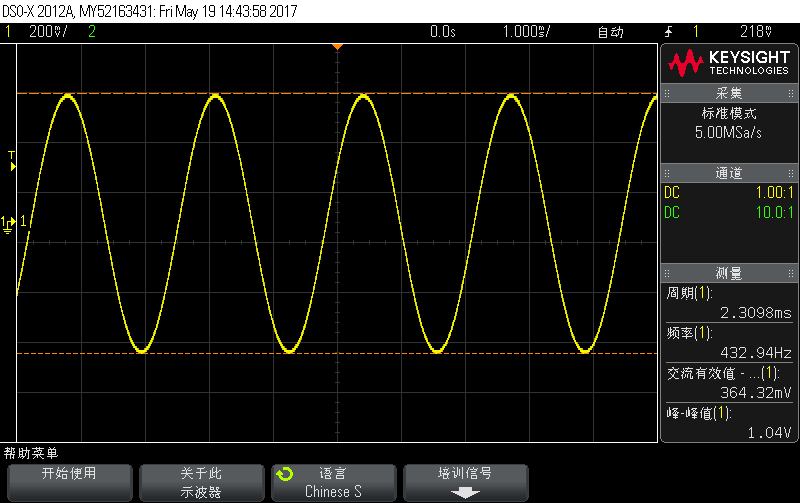
\includegraphics[width=\textwidth]{scope_1.png}
\end{figure}
输出电压的峰-峰值为$1.04V$,频率为$432.94Hz$。
\subsubsection{调整$R_w$使输出为不失真的正弦波且幅值最大,记录$U_o$幅值、频率及$R_w$的阻值}
输出不失真且幅值最大时,用万用表电阻档测得$R_w = 18.12k\Omega$,波形如下:
\begin{figure}[H]
\centering
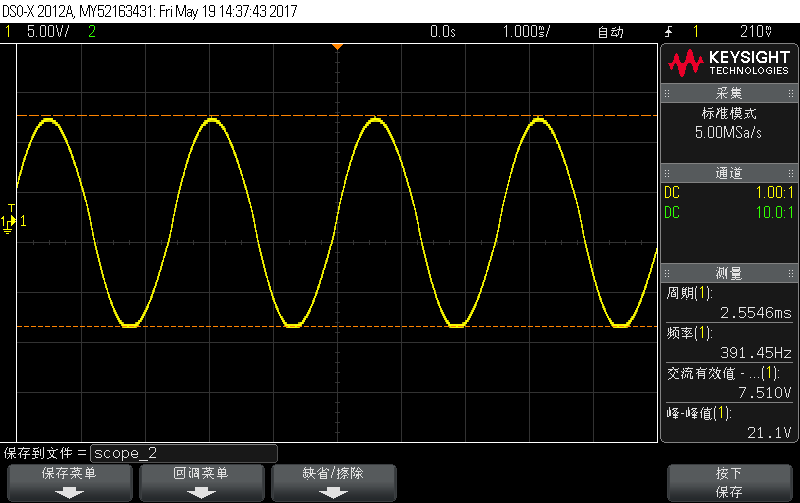
\includegraphics[width=\textwidth]{scope_2.png}
\end{figure}
输出电压的峰-峰值为$21.1V$,频率为$391.45Hz$。
\subsubsection{将两个二极管断开,观察$R_w$从小到大变化时输出波形的变化情况}
$R_w$从小变大的过程中,首先输出端没有振荡波形;随后刚刚起振波形峰-峰值就非常大。如下图所示:
\begin{figure}[H]
\centering
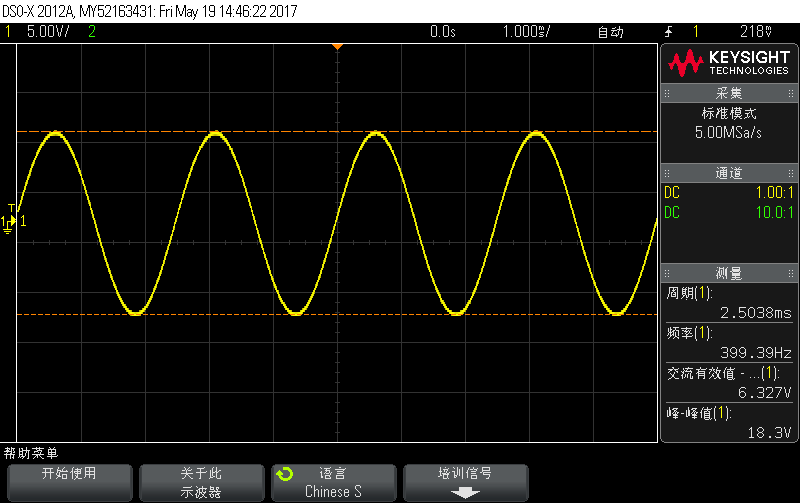
\includegraphics[width=\textwidth]{scope_3-1.png}
\end{figure}
随后稍微增大,即出现明显失真。波形如下:
\begin{figure}[H]
\centering
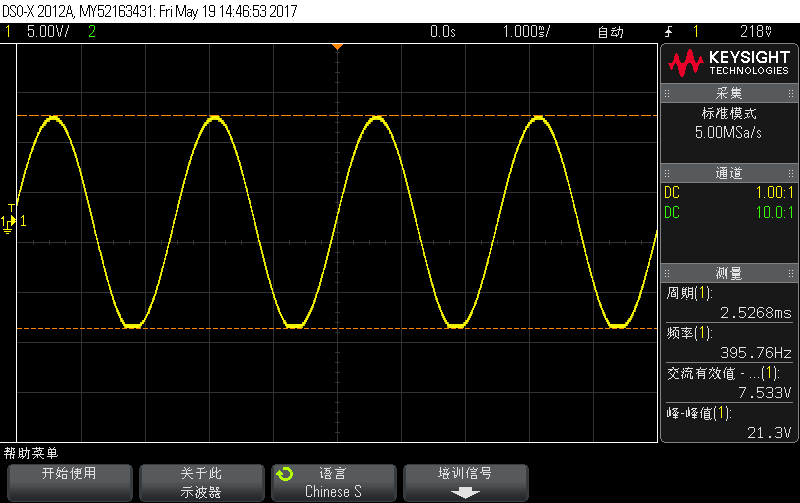
\includegraphics[width=\textwidth]{scope_3-2.png}
\end{figure}
可以看到,没有二极管非线性稳幅,运算放大器输出非常容易饱和,正弦波非常容易失真,这充分说明了稳幅环节对于正弦波发生电路的重要性。
\subsubsection{总结}
\begin{table}[H]
\centering
\begin{tabular}{|c|c|c|c||c|c|c|c|}
\hline 
起振&$R_{w}(k\Omega)$ & $U_op-p(V)$ & $f_o(Hz)$ &幅值最大&$R_{w}(k\Omega)$ & $U_op-p(V)$ & $f_o(Hz)$\\ \hline 
仿真数据&$10.4$ & $2.918$ & $400$ &仿真数据&$18.0$ & $20.736$ & $400$ \\ \hline
实验测量&$9.91$& $1.04$ &  $432.94$& 实验测量&$18.12$& $21.1$ &  $391.45$\\ \hline 
\end{tabular} 
\end{table}
可以看到,仿真值与实验值除了起振电压外均相当接近。这一差异可以解释为,仿真进行的是数值计算,时间远长于实验,因此仿真有时为了等待时间不至于过长可能会人为地调大起振时$R_w$值,也就增大了$U_o$。表格中可以看到,随着$R_w$的增大,输出正弦波的频率将会下降,这是由于$R、C$取值不够理想导致的,后面将介绍的实验中遇到的问题有一个即与此相关。
\subsection{矩形波-三角波发生电路}
测量$u_{o1}$、$u_{o2}$波形的幅值、周期及$u_{o2}$的正程、逆程时间。\par
示波器波形为:
\begin{figure}[H]
\centering
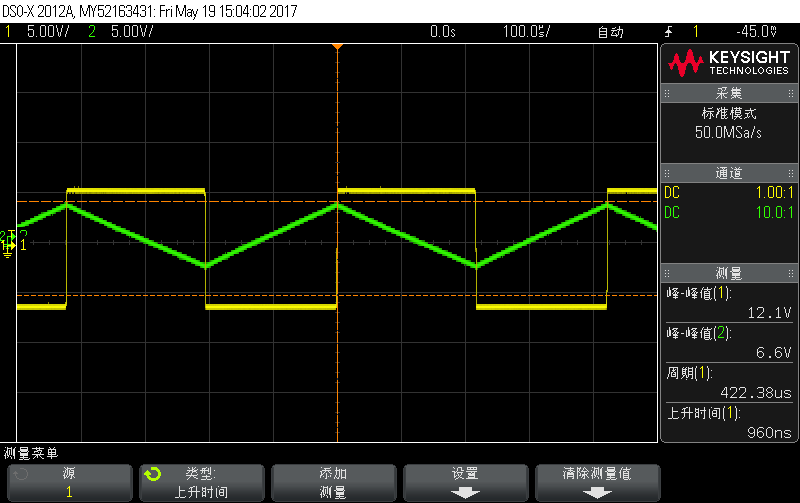
\includegraphics[width=\textwidth]{scope_4.png}
\end{figure}
可以看到,$u_{o1}$为方波,峰-峰值为$12.1V,u_{o2}$为三角波,峰-峰值为$6.6V$,周期为$422.38\mu s$。\\
更精细地,如下图所示用游标测量正程、逆程时间,示波器显示如下:
\begin{figure}[H]
\centering
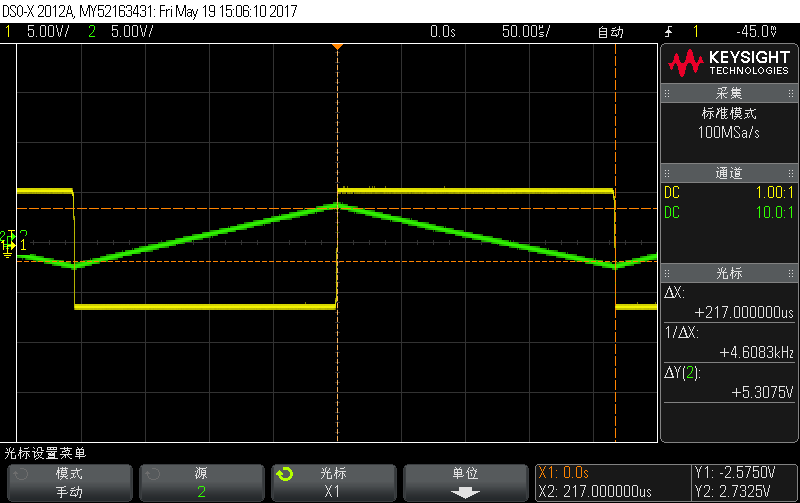
\includegraphics[width=\textwidth]{scope_5.png}
\end{figure}
测得$u_{o2}$的正程时间为$205\mu s$,逆程时间为$217\mu s$,这反映出实际元件参数的不对称。\par
将理论、仿真与实验结果总结如下:
\begin{table} [H]
\centering
\begin{tabular}{|c|c|c|c|c|c|}
\hline 
&$U_{o1p-p}(V)$ &$U_{o2p-p}(V)$ &$ T(\mu s)$ &$t_{正程}(\mu s)$ &$t_{逆程}(\mu s)$\\ \hline 
理论值 &$11.6$ &$5.8$ &$400$ &$ 200$ &$200$ \\ \hline
仿真数据&$12.581$& $6.398$ &$418$ & $208.955$ &$208.955$\\ \hline 
实验测量&$12.1$ & $6.6$ & $422.38$ &$205$ &$217$ \\ \hline
\end{tabular} 
\end{table}
可以看到,三者相当接近,差异主要是稳压管的导通压降和实际元件参数的不对称性导致的。
\subsection{滞回比较器的电压传输特性}
\begin{figure}[H]
\centering
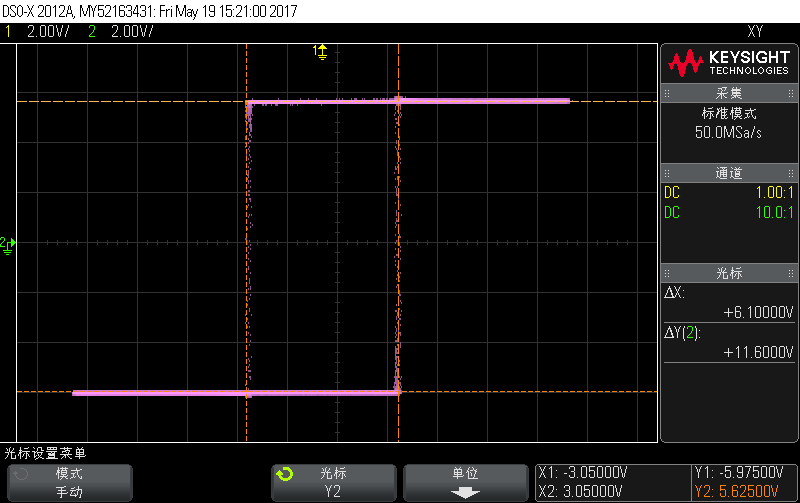
\includegraphics[width=0.7\textwidth]{scope_7.png}
\end{figure}
用游标测得阈值电压为$\pm 3.05V$,$u_{o1}$的峰-峰值为$11.60V$。将理论、仿真、实验值整理如下。
\begin{table}[H]
\centering
\begin{tabular}{|c|c|c|c|c|}
\hline 
&$U_T(V)$ &$-U_T(V)$& $u_{o1+}(V)$ &$u_{o1-}(V)$\\ \hline 
理论值 &$2.9$ &$-2.9$ &$5.8$ &$-5.8$ \\ \hline
仿真数据&$3.296$& $-3.358$ &  $6.310$& $-6.311$\\ \hline 
实验测量&$3.05$ & $-3.05$ & $5.625$ &$-5.975$ \\ \hline
\end{tabular} 
\end{table}
可以看到,三者比较接近。原因与矩形波-三角波发生电路相同。其中仿真、实验与理论值的差异,很大程度上是稳压管的导通压降导致的;而实际电路中又存在元件不可能理想对称的问题。
\subsection{矩形波-锯齿波发生电路}
波形如下所示。
\begin{figure}[H]
\centering
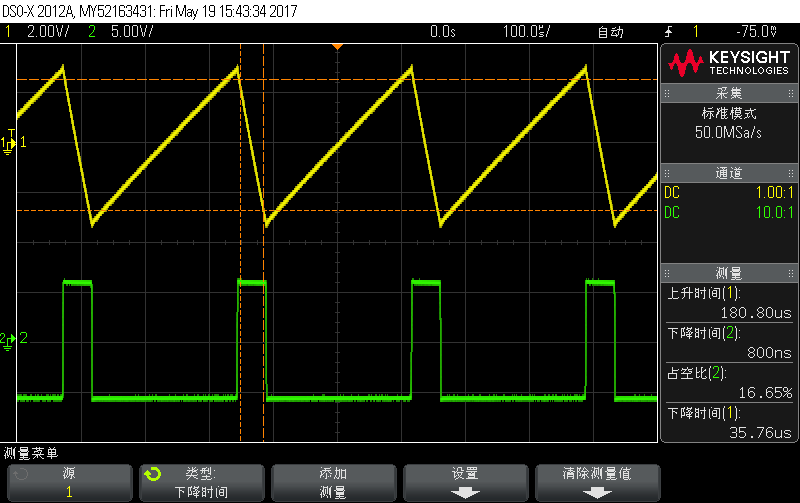
\includegraphics[width=\textwidth]{scope_9.png}
\end{figure}
由于数值有上下波动,实验记录的平均值与截图值稍有不同。最终占空比为$16.66\%$,正程时间$181.50\mu s$,逆程时间$36.20\mu s$,逆程时间是正程时间的$19.94\%$,更进一步地,测得周期为$272.44\mu s$,$U_{o1}$的峰-峰值$12.0V$,$U_{o2}$的峰-峰值$6.48V$。\par
总结如下:
\begin{table} [H]
\centering
\begin{tabular}{|c|c|c|c|}
\hline 
&$U_{o1p-p}(V)$ &$U_{o2p-p}(V)$ &$ T(\mu s)$\\ \hline 
仿真数据&$12.126$&$6.508$&$284.091$\\ \hline
实验测量&$12.0$&$6.48$&$272.44$\\ \hline
\end{tabular}
\end{table}
可以看到,二者相当接近。
\section{实验中遇到的问题及解决方法}
\subsection{仿真时运算放大器输出值大于供电电压的问题}
这个问题在实验前的仿真终于到,对于本次全部四项实验均构成了影响,其真正解决是在实验完成以后。\par
“喷泉的高度不会超过它的源头”\footnote{林肯语},运算放大器的输出电压在实际中不会高过直流供电电源的电压,但是在仿真时却出现了输出电压达几十$kV$、甚至更高的情况。这导致了正弦波发生电路中$R_w$不论多大均不失真;矩形波-三角波发生电路虽然产生了矩形波和三角波,但周期是$0.4ms$的十倍,因而对矩形波-锯齿波电路也造成了影响;而对于滞回比较器,则输出始终为负,并不跳变。这里将矩形波-三角波的波形截图如下。
\begin{figure}[H]
\centering
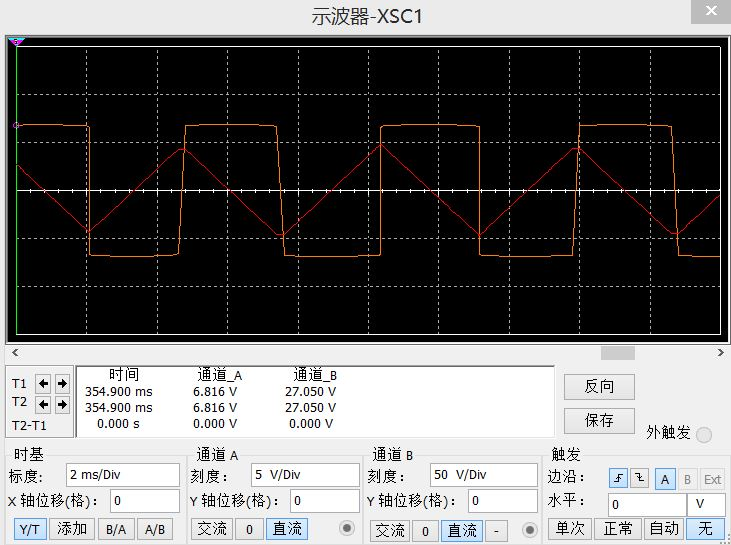
\includegraphics[width=\textwidth]{9.jpg}
\end{figure}
可以看到,其周期在$4ms$左右。\par
这一问题令我十分困惑,为此更换了各种LF347(包括BD、D、N)都无法解决。最终的解决还是在实验完成以后,发现问题在于厂家的选择,我特意选择了IIT厂家的器件,而若使用Texas Instrument的器件则不存在此问题。\par
这个问题最后导致我仿真重新做了一遍,个人认为这样的问题很不科学,应该是仿真模型的问题。
\subsection{仿真时三角波、滞回比较器波形不好的问题}
这个问题体现为在示波器直流耦合的情况下三角波仍然会显得波形不规则、滞回比较器的传输特性仍然不能直上直下而是明显地倾斜。第一个问题是由于我自己选择了厂家导致,同学没有遇到这一问题。相比于此,这第二个问题是同学们普遍遇到的。\par
这一问题的解决也是在实验后,最后通过与电机系同学进行交流解决。设置Multisim中仿真->交互仿真设置->步长,将步长减小,如减小到$10^{-5}或10^{-6}$即可解决这一问题。这是由于,仿真的更加精密,可使仿真结果更符合实际,当然代价就是需要花费更多时间。
\subsection{实验中增大$R_w$后频率大幅降低的问题}
实验中,我最初的$R_1、C_1$选择与仿真时一致。在起振时,频率还正常,为$403.55Hz$,如下图所示。
\begin{figure}[H]
\centering
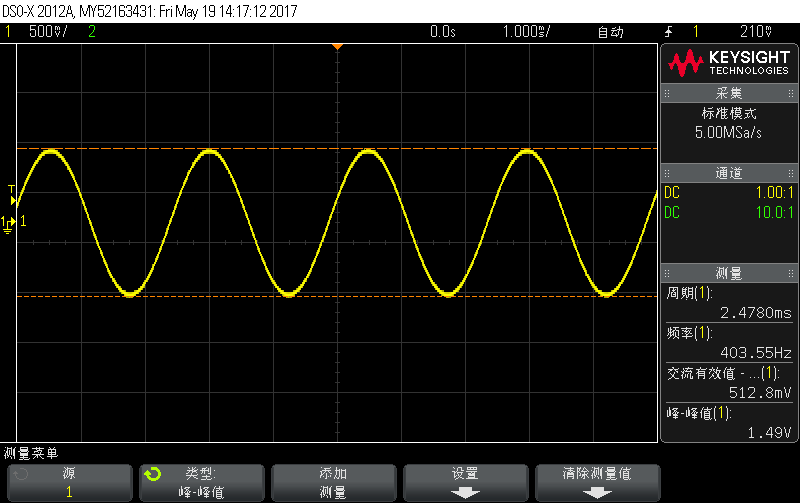
\includegraphics[width=\textwidth]{scope_1-.png}
\end{figure}
但在增大$R_w$后,频率居然降为$356.15Hz$,如下图所示。
\begin{figure}[H]
\centering
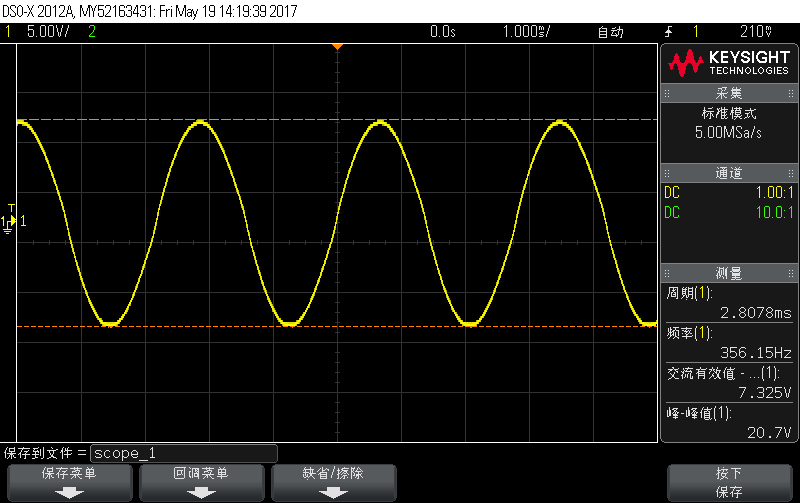
\includegraphics[width=\textwidth]{scope_2-.png}
\end{figure}
这一问题是由于$R_1$阻值选择偏小造成的。后来更换为$R_1=12k\Omega,C_1=33nF$,仍不能解决这一问题(这大概还存在电阻、电容值与标称值有偏差的问题),最后选择$R_1=39k\Omega,C=10nF$,才得到前面实验报告中的波形。
\subsection{实验中按理论电阻值接入不能实现$t_f=20\% t_r$的问题}
这一问题再次体现了实际器件与理想器件参数的差异。使用与理论值相同的$4k\Omega$电阻时,测得$U_{o1p-p} = 12.3V,U_{o2p-p} = 6.5V,T=272.45\mu s$,此时$\frac{t_f}{t_r} = \frac{54}{224}=24.1\%$。如果增大这一电阻值,理论上,应使这一比例增大,但实际上,换为$4.4k\Omega$的电阻后,却发现这一比例变为$\frac{52}{230}=22.6\%$,这再次反映了实际器件参数可能的不准确。\par
最后在秦俭老师的鼓励下,使用滑动变阻器对这一合适阻值进行探究,以占空比$16.67\%$为指标进行调节,最终在该电阻取值为$3.51k\Omega$时,得到了满意的结果,如前面实验报告所示。
\section{实验体会}
这次实验虽然遇到了一些问题,但是最终在一节课上当堂完成,令我很有满足感。体会主要有以下四点。\par
\begin{enumerate}
\item 对于正弦波发生电路、滞回比较器、矩形波-三角波发生电路的原理理解更加到位,特别是对正弦波发生电路中参数选择对实际电路性能的影响有了更深入的理解。
\item 本次仿真实验花费的时间实际上要远长于实际搭电路的时间,这主要是由于Multisim模型的一些问题和自己对于Multisim的使用掌握尚不够深入。通过这次实验,自己对Multisim的使用更加熟悉。这对于未来的EDA工作是非常有价值的。
\item 本次实验同样让我看到了理论与实际的差距。分立元件不仅可能与标称值存在较大偏差,而且其元件与元件之间并没有理想的相同特性,这说明了在工程问题中考虑容差范围的重要性。
\item 最后,这次实验的仿真和硬件实验过程中,与老师和同学的交流都使我受益良多,这种讨论学习的方式也使得电路课程的学习不显得那么枯燥无味。在此对他们一并表示感谢。
\end{enumerate}
\end{spacing}
\end{document}
